%%%%%%%%%%%%%%%%%%%%%%%%%%%%%%%%%%%%%%%%%%%%%%%%%%%%%%%%%%%%%%%%%%%%%%%%%%%%%%%%%%
\begin{frame}[fragile]\frametitle{}
\begin{center}
{\Large Model Context Protocol (MCP)}
\end{center}
\end{frame}

%%%%%%%%%%%%%%%%%%%%%%%%%%%%%%%%%%%%%%%%%%%%%%%%%%%%%%%%%%%
\begin{frame}[fragile]\frametitle{LLMs Alone Aren't Enough}

\begin{columns}
    \begin{column}[T]{0.5\linewidth}
      \begin{itemize}
        \item Real AI apps need search, tools, memory, and APIs
        \item LLMs can't handle complex tasks on their own
        \item Integration quickly becomes messy and fragile
      \end{itemize}

    \end{column}
    \begin{column}[T]{0.5\linewidth}
		\begin{center}
		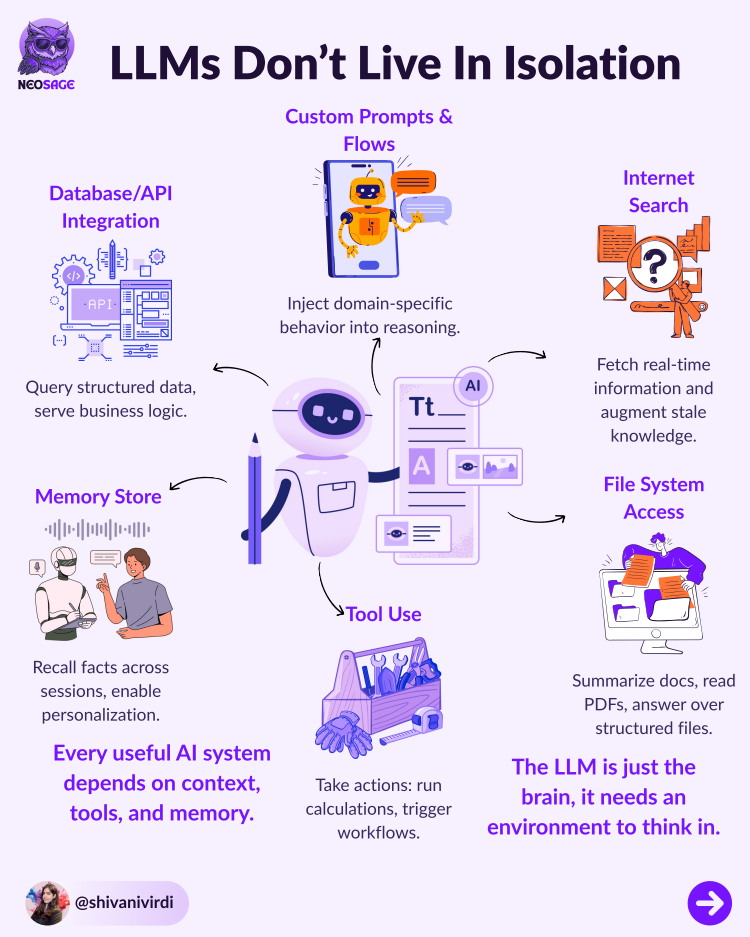
\includegraphics[width=\linewidth,keepaspectratio]{aiagents9}
		\end{center}
    \end{column}
  \end{columns}
   
\end{frame}


%%%%%%%%%%%%%%%%%%%%%%%%%%%%%%%%%%%%%%%%%%%%%%%%%%%%%%%%%%%
\begin{frame}[fragile]\frametitle{The Integration Problem}

\begin{columns}
    \begin{column}[T]{0.5\linewidth}
      \begin{itemize}
        \item Every feature requires custom wrappers
        \item Updates often break existing logic
        \item M apps $\times$ N tools = scaling nightmare
      \end{itemize}

    \end{column}
    \begin{column}[T]{0.5\linewidth}
		\begin{center}
		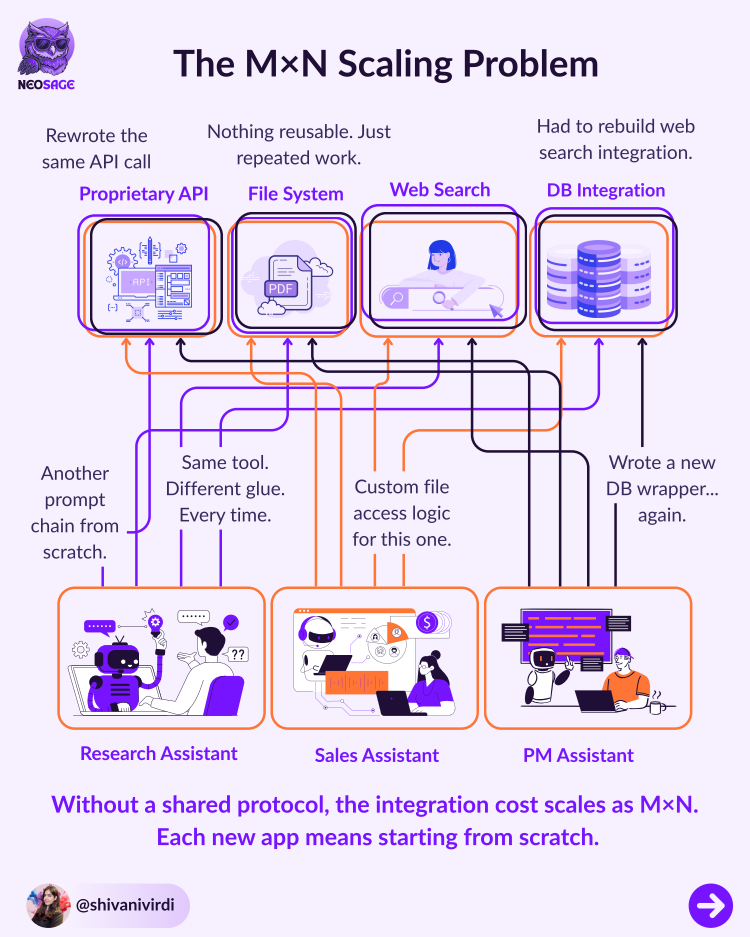
\includegraphics[width=\linewidth,keepaspectratio]{aiagents11}
		\end{center}
    \end{column}
  \end{columns}
  
\end{frame}

%%%%%%%%%%%%%%%%%%%%%%%%%%%%%%%%%%%%%%%%%%%%%%%%%%%%%%%%%%%
\begin{frame}[fragile]\frametitle{Enter MCP: USB-C for AI}
\begin{columns}
    \begin{column}[T]{0.5\linewidth}
      \begin{itemize}
        \item Shared protocol for AI-to-tool connections
        \item One-time tool exposure works with all models
        \item No wrappers, less chaos, easy reuse
      \end{itemize}

    \end{column}
    \begin{column}[T]{0.5\linewidth}
		\begin{center}
		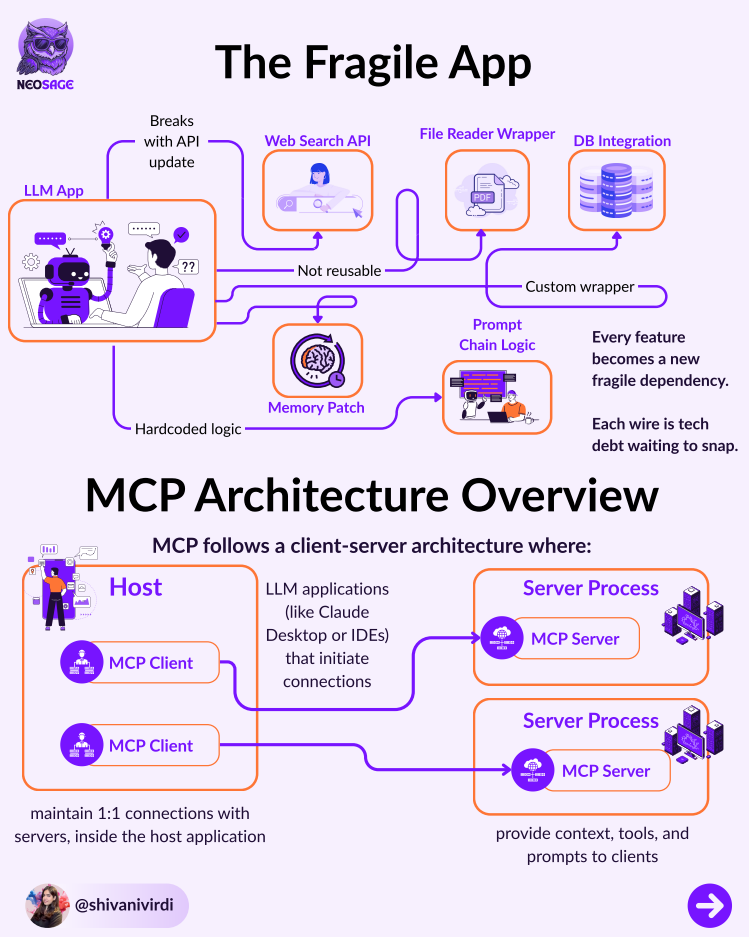
\includegraphics[width=\linewidth,keepaspectratio]{aiagents10}
		\end{center}
    \end{column}
  \end{columns}
\end{frame}


%%%%%%%%%%%%%%%%%%%%%%%%%%%%%%%%%%%%%%%%%%%%%%%%%%%%%%%%%%%
\begin{frame}[fragile]\frametitle{How MCP Works?}
\begin{columns}
    \begin{column}[T]{0.5\linewidth}
      \begin{itemize}
        \item Host: the AI app (e.g., Claude Desktop)
        \item Client: bridge that speaks MCP
        \item Server: where tools, files, prompts live
      \end{itemize}

    \end{column}
    \begin{column}[T]{0.5\linewidth}
		\begin{center}
		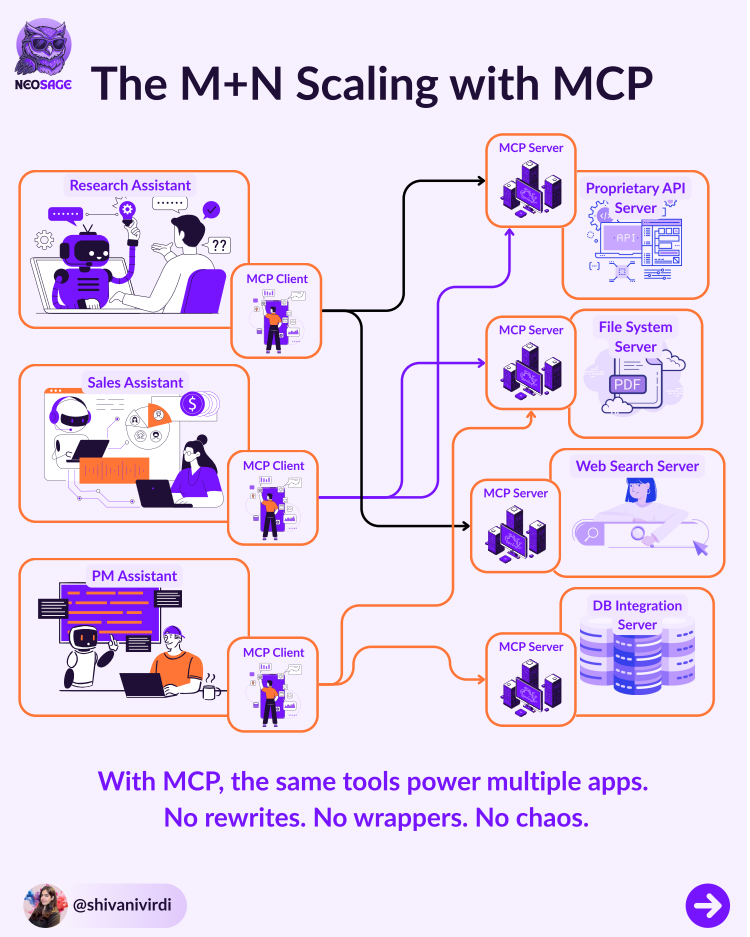
\includegraphics[width=\linewidth,keepaspectratio]{aiagents12}
		\end{center}
    \end{column}
  \end{columns}
\end{frame}

%%%%%%%%%%%%%%%%%%%%%%%%%%%%%%%%%%%%%%%%%%%%%%%%%%%%%%%%%%%
\begin{frame}[fragile]\frametitle{Clean, Typed Communication}
\begin{columns}
    \begin{column}[T]{0.5\linewidth}
      \begin{itemize}
        \item Uses JSON-RPC for structured messaging
        \item Modular design enables reuse
        \item Protocol simplifies complex system behavior
      \end{itemize}

    \end{column}
    \begin{column}[T]{0.5\linewidth}
		\begin{center}
		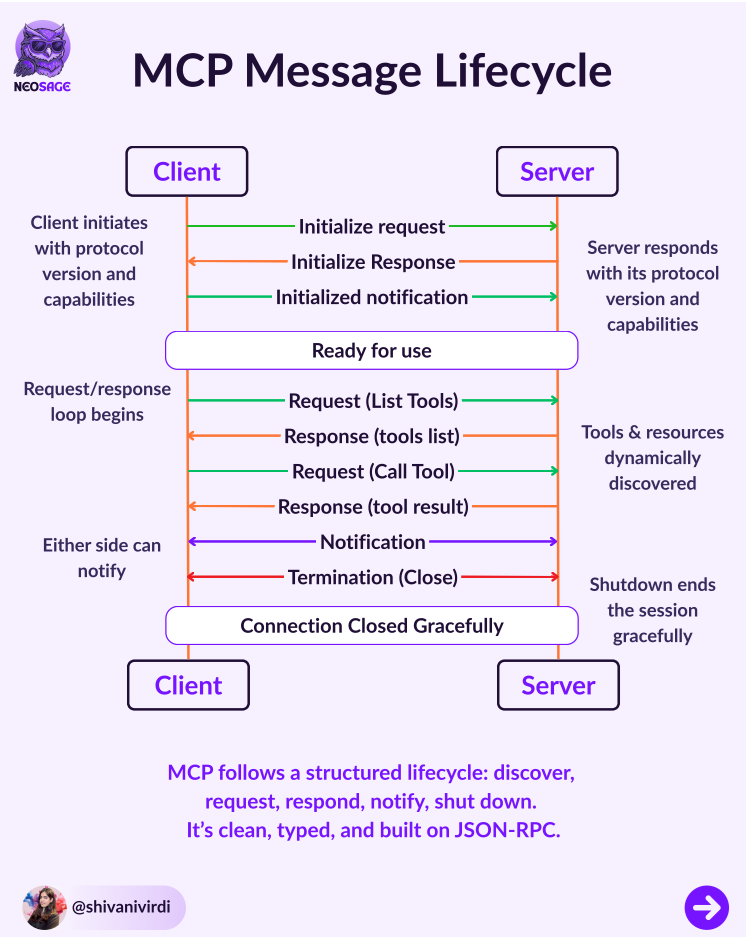
\includegraphics[width=\linewidth,keepaspectratio]{aiagents13}
		\end{center}
    \end{column}
  \end{columns}
\end{frame}

%%%%%%%%%%%%%%%%%%%%%%%%%%%%%%%%%%%%%%%%%%%%%%%%%%%%%%%%%%%
\begin{frame}[fragile]\frametitle{From Demos to Real Systems}

\begin{columns}
    \begin{column}[T]{0.5\linewidth}
      \begin{itemize}
        \item MCP transforms fragile demos into scalable systems
        \item Reduces engineering overhead
        \item Enables AI software that ships and lasts
      \end{itemize}

    \end{column}
    \begin{column}[T]{0.5\linewidth}
		\begin{center}
		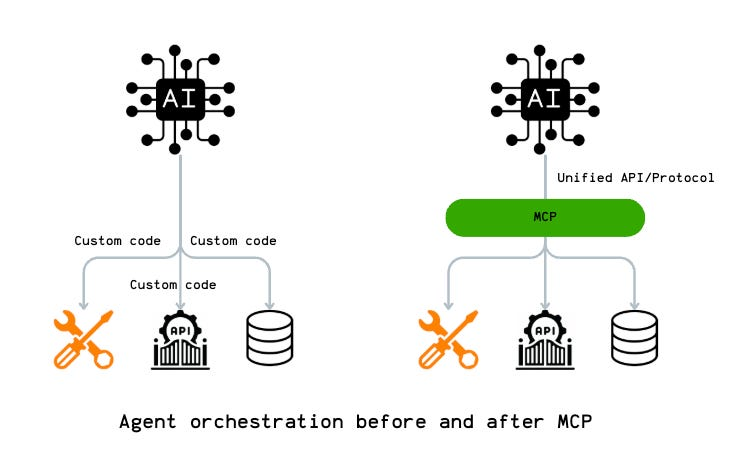
\includegraphics[width=\linewidth,keepaspectratio]{aiagents17}
		
		{\tiny (Ref: Agentic AI For Everyone - Aish \& Kiriti)}
		\end{center}
    \end{column}
  \end{columns}
  
	
\end{frame}

%%%%%%%%%%%%%%%%%%%%%%%%%%%%%%%%%%%%%%%%%%%%%%%%%%%%%%%%%%%
\begin{frame}[fragile]\frametitle{So, what is MCP?}
      \begin{itemize}
        \item A standardized way to deliver full context to an LLM
        \item Includes task, tools, memory, documents, and prior messages
        \item Acts like a structured input package for the model
        \item Similar to protocols like HTTP or TCP/IP — not a product
        \item Enables clean communication between model and system
      \end{itemize}
\end{frame}

%%%%%%%%%%%%%%%%%%%%%%%%%%%%%%%%%%%%%%%%%%%%%%%%%%%%%%%%%%%
\begin{frame}[fragile]\frametitle{Why MCP Matters}
      \begin{itemize}
        \item Avoids reinventing prompt logic for every use case
        \item Standardizes context delivery for agents
        \item Simplifies managing memory, tools, and state
        \item Enables modular, composable orchestration
        \item Think of it as a structured request schema for LLMs
      \end{itemize}
\end{frame}

%%%%%%%%%%%%%%%%%%%%%%%%%%%%%%%%%%%%%%%%%%%%%%%%%%%%%%%%%%%
\begin{frame}[fragile]\frametitle{How MCP Helps in Practice}
      \begin{itemize}
        \item Reduces chaos in multi-tool, multi-context systems
        \item Makes integration with RAG, memory, and outputs cleaner
        \item Easier to plug agents into enterprise pipelines
        \item Moves away from dumping long prompts into the model
        \item Structured text input improves grounding and clarity
      \end{itemize}
\end{frame}

%%%%%%%%%%%%%%%%%%%%%%%%%%%%%%%%%%%%%%%%%%%%%%%%%%%%%%%%%%%
\begin{frame}[fragile]\frametitle{Why MCP Gained Traction}
      \begin{itemize}
        \item AI-native: designed for agents, tools, memory, and more
        \item Strong initial documentation and real examples
        \item Released SDKs, testing tools, and demos
        \item Quiet launch in 2024; exploded in 2025 adoption
        \item Broad support from OpenAI, startups, and platforms
      \end{itemize}
\end{frame}

%%%%%%%%%%%%%%%%%%%%%%%%%%%%%%%%%%%%%%%%%%%%%%%%%%%%%%%%%%%
\begin{frame}[fragile]\frametitle{Common Misunderstandings}
      \begin{itemize}
        \item MCP is not a new API or product
        \item It doesn’t make models smarter — just clearer context
        \item Useful beyond agents — assistants benefit too
        \item Helps structure evolving context, not static prompts
      \end{itemize}
\end{frame}

%%%%%%%%%%%%%%%%%%%%%%%%%%%%%%%%%%%%%%%%%%%%%%%%%%%%%%%%%%%
\begin{frame}[fragile]\frametitle{Should You Care About MCP?}
      \begin{itemize}
        \item Not essential for simple demos or toy prompts
        \item Crucial for enterprise-grade agent systems
        \item Helps with multi-tool, RAG, memory, and planning workflows
        \item Improves long-term context management and scale
        \item Adoption is key — like any protocol, usage defines value
      \end{itemize}
\end{frame}




%%%%%%%%%%%%%%%%%%%%%%%%%%%%%%%%%%%%%%%%%%%%%%%%%%%%%%%%%%%
\begin{frame}[fragile]\frametitle{MCP: From Demos to Real Systems}

\begin{columns}
    \begin{column}[T]{0.5\linewidth}
		\begin{center}
		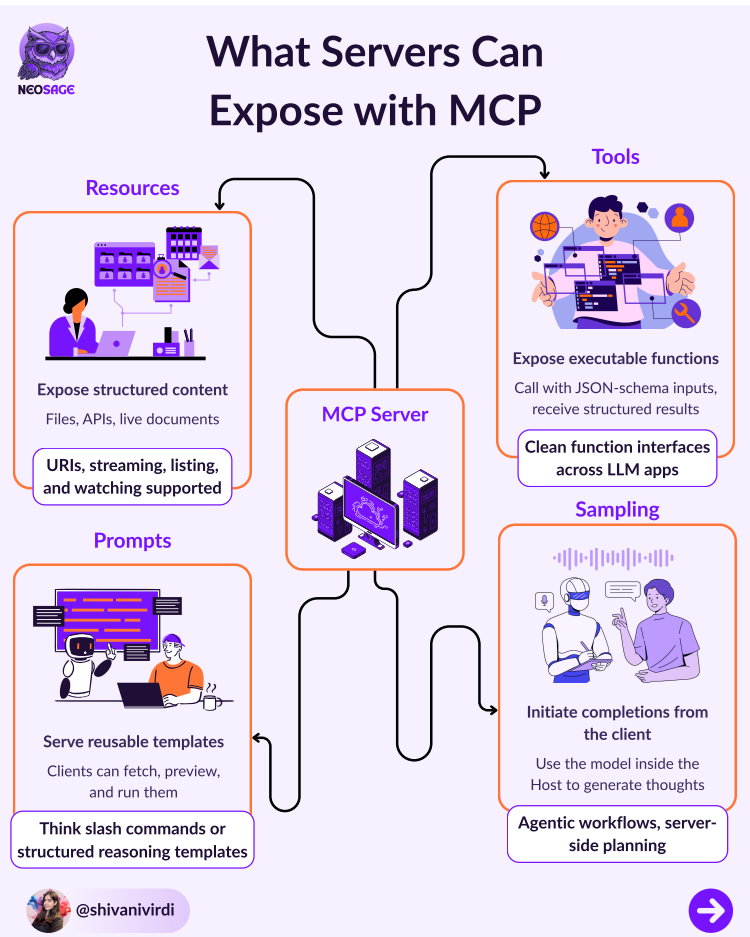
\includegraphics[width=\linewidth,keepaspectratio]{aiagents14}
		\end{center}

    \end{column}
    \begin{column}[T]{0.5\linewidth}
		\begin{center}
		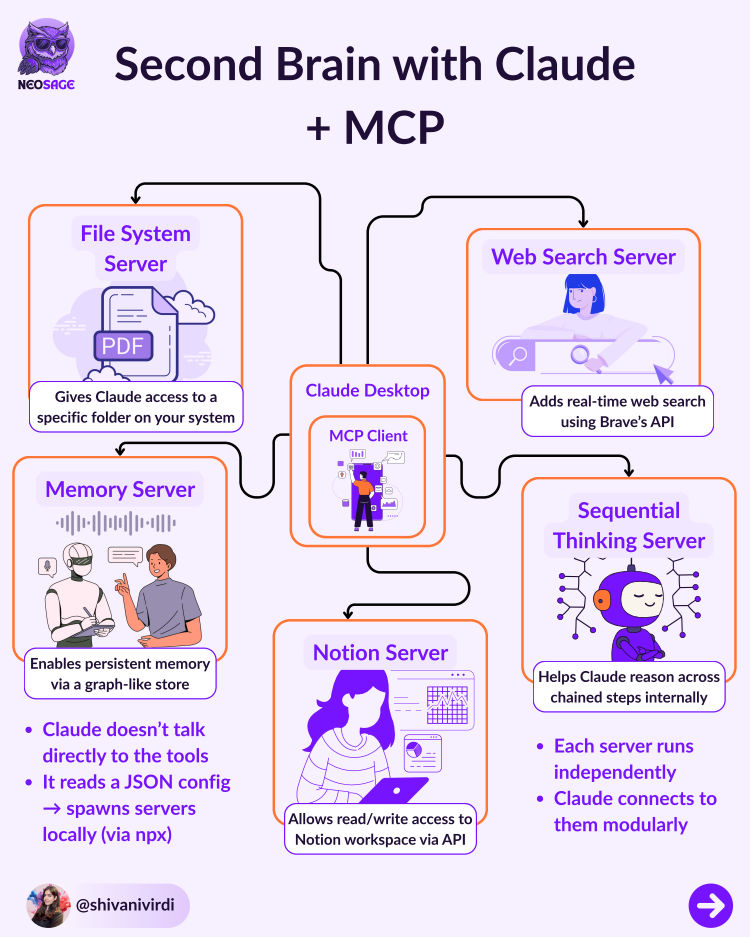
\includegraphics[width=\linewidth,keepaspectratio]{aiagents15}
		\end{center}
    \end{column}
  \end{columns}
  


\end{frame}

%%%%%%%%%%%%%%%%%%%%%%%%%%%%%%%%%%%%%%%%%%%%%%%%%%%%%%%%%%%
\begin{frame}[fragile]\frametitle{Some Opposition to MCP \ldots}
    \begin{itemize}
        \item Fancy acronyms often solve imaginary problems
        \item Overengineered MCP layers complicate agent-API flow
        \item Hype drives architecture-not actual needs
        \item Direct API calls are faster and clearer
        \item Lower latency and reduced system complexity
        \item Easier to debug, scale, and maintain	
		\item Skip the MCP if your API already works
        \item Avoid unnecessary layers for trend's sake
        \item Prioritize shipping over architecture theater
    \end{itemize}
\end{frame}


%%%%%%%%%%%%%%%%%%%%%%%%%%%%%%%%%%%%%%%%%%%%%%%%%%%%%%%%%%%%%%%%%%%%%%%%%%%%%%%%%%
\begin{frame}[fragile]\frametitle{}
\begin{center}
{\Large Zerodha Kite MCP Server}
\end{center}
\end{frame}
